\section{Application: Finding extensions of underconstrained glassy structures to isostatic}
\label{sec:bodypin}

We can use DR-plans to help in solving questions in designs for graphene and silica bilayers (\todo{Add Citation}). Specifically, we will look into the problem when you have a monolayer and it is underconstrained. Our goal is to make such a layer isostatic. This can be done in a number of ways.

\begin{figure}\centering
    \includegraphics[width=0.4\linewidth]{img/Silica} \hspace{0.5cm}
    \raisebox{0.5\height}{\includegraphics[width=0.2\linewidth]{img/Silicon_tetrahedron}}
    \caption{Example of a signle layer of a Silica Oxygen glassy structure. This can be thought of as a multi-triangle-pin qusec where the Silicon atoms are the triangles and the Oxygen atoms are the pins. Not shown here are other layers stacked on this one. Each Silicon atom has the structure seen to the right, and so binds to another Oxygen atom in another layer.}
    \label{fig:silica_glass}
\end{figure}

\begin{itemize}
    \item Pin together 2 underconstrained monolayers in such a way that the resulting bilayer becomes isostatic (see Figure \ref{fig:silica_glass}).
    \item Pin the boundary in such a way that the resulting system is isostatic.
    \item Build the structures by repeated subdivision to ensure they are isostatic at each layer (see Figure \ref{fig:subdivision})
\end{itemize}

We will discuss item 2 in detail in this section. In each case, we are specifically interested in how to they can be applied to get a resulting isostatic structure with a small DR-plan, so a realization can be found quickly. To answer these questions, we first inroduce the structures we model the problems with:

\begin{figure}\centering
    \begin{subfigure}{0.25\linewidth}
        \includegraphics[width=\linewidth]{img/pentl1}
    \end{subfigure}
    % 
    \begin{subfigure}{0.25\linewidth}
        \includegraphics[width=\linewidth]{img/pentl2}
    \end{subfigure}
    % 
    \begin{subfigure}{0.4\linewidth}
        \includegraphics[width=\linewidth]{img/pentl3}
    \end{subfigure}
    \caption{An example of self-similarity in the form of repeated subdivisions. Each figure follows fromt he previous due to a set subdivision rule. If each figure was guaranteed to be isostatic, then isostatic systems of arbitrary detail could be made.}
    \label{fig:subdivision}
\end{figure}

\subsection{Body-Pin}


\begin{definition}
    A multi-body-pin qusec is a qusec where the obejct are rigid bodies that are pinned together by some number of pins.
\end{definition}

\begin{remark}
    A multi-body-pin qusec is a special case of bar-joint qusecs that we have been studying. As such, the DR-planning discussed in Section \ref{sec:DRP} is unchanged and the work in Section \ref{sec:recomb} will still go through with slight modifications.
\end{remark}

\begin{proof}
    We can replace each body that has only one pin by a single vertex. A body with 2 pins can be replaced by an edge. In general, a body with $n$ pins can be replaced by a 2-tree on $n$ vertices. When looking for a DR-plan, we treat each body as trivial, so they become the leaves of our plan. The optimal completion problem and approach of Section \ref{sec:DRP} are unchanged. The optimal paramaterization problem in Section \ref{sec:DRP} now has an additional constraint that all edges in the 2-tree representation of the bodies must be removed together, not individually.
\end{proof}

We now go over 2 subclasses of multi-body-pin qusecs for modeling Examples 4 and 5 in Section \ref{sec:intro}.

\begin{definition}
\label{def:body-pin}
    A body-pin qusec is a multi-body-pin qusec with the following conditions:
    \begin{itemize}
        \item Each pin is shared by at most 2 bodies
        \item No 2 bodies share more than one pin
    \end{itemize}
    Such a body-pin qusec can also be seen as a {\em body-bar graph} where the bodies are the original bodies and each pin represents 2 bars from one body to another. For such body-bar qusecs, graphs with 1 and 2 dofs can be characterized by being $(3,4)$ and $(3,5)$-tight respectively.
\end{definition}

\begin{definition}
    A multi-triangle-pin qusec is a multi-body-pin qusec where each body is a triangle, meaning it is pinned in at most 3 places. This is also represented as a hyper-graph where each pin is a vertex and each triangle represents a tri-hyperedge. For such hyper-graphs, 1 and 2 dofs can be characterized by $(2,4)$ and $(2,5)$ tightness respectively.
\end{definition}

Body-pin qusecs are of particular interest to us in the context of Example 4 in Section \ref{sec:intro}. Multi-triangle-pin qusecs can be used to reprsent the silica bi-layers and glassy structures described in Example 5 of Section \ref{sec:intro}, where each triangle is the junction of ``disks'' in the plane (se Figure \ref{fig:silica_glass}). Typically, these systems are not isostatic, so to relate the work of this paper to the systems, we define a slightly different kind of DR-plan:

\begin{definition}
    A $(k,l)$-tight DR-plan is one in which each child node is either a vertex maximal proper $(k,l)$-tight subgraph of the parent node or it is trivial. In our case, the trivial nodes are just the bodies.
\end{definition}

We can develop the notion of a canonical DR-plan for certain $(k,l)$ tightness conditions similar to the way we did in Section \ref{sec:DRP}.

\begin{remark}
\label{rem:1dofcanon}
    For the 1 dof multi-body-pin qusecs described above, a DR-plan node will follow one of the following:

    \begin{itemize}
        \item Its children will be 2 proper vertex maximal 1 dof graphs that intersect on another 1 dof graph
        \item Its children will be a number of proper maximal 1 dof subgraphs, joined pairwise by at most one pin
    \end{itemize}
\end{remark}

\begin{proof}
    \todo{Item 1 Follows from paper?}

    For item 2, consider the case where we have more than 2 proper vertex maximal 1 dof subgraphs $s_1, ..., s_k, k > 2$. Then, if $k_i$ and $k_j$ are joined by $2$ pins, $k_i \Cup k_j$ would be $(3,4)$-tight and hence $k_i$ and $k_j$ are not vertex maximal.
\end{proof}

\begin{remark}
    All $(k,l)$-tight canonical DR-plans are optimal. We can find such a DR-plan in the same time complexity as the $(2,3)$ tight case for bar and joint qusecs discussed in Section \ref{sec:DRP}.
\end{remark}

\begin{figure*}\centering
\begin{subfigure}{0.2\linewidth}\centering
    \includegraphics[width=\linewidth]{img/bodypin}
    \caption{}
\end{subfigure}
%
\begin{subfigure}{0.2\linewidth}\centering
    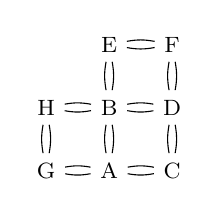
\begin{tikzpicture}[scale=0.8]
    % \tikzstyle{v}=[draw, circle, minimum size=0.1cm, scale=0.7, font=\footnotesize]
    \tikzstyle{v}=[font=\footnotesize]

    \node[v] (a) at (0,0) {A};
    \node[v] (b) at (0,1) {B};
    \node[v] (c) at (1,0) {C};
    \node[v] (d) at (1,1) {D};
    \node[v] (e) at (0,2) {E};
    \node[v] (f) at (1,2) {F};
    \node[v] (g) at (-1,0) {G};
    \node[v] (h) at (-1,1) {H};

    \draw (a) to [bend right=10](b);
    \draw (a) to [bend left=10](b);
    \draw (a) to [bend right=10](c);
    \draw (a) to [bend left=10](c);
    \draw (d) to [bend right=10](c);
    \draw (d) to [bend left=10](c);
    \draw (b) to [bend right=10](d);
    \draw (b) to [bend left=10](d);
    \draw (b) to [bend right=10](e);
    \draw (b) to [bend left=10](e);
    \draw (b) to [bend right=10](h);
    \draw (b) to [bend left=10](h);
    \draw (g) to [bend right=10](h);
    \draw (g) to [bend left=10](h);
    \draw (g) to [bend right=10](a);
    \draw (g) to [bend left=10](a);
    \draw (f) to [bend right=10](e);
    \draw (f) to [bend left=10](e);
    \draw (f) to [bend right=10](d);
    \draw (f) to [bend left=10](d);
\end{tikzpicture}
    \caption{}
\end{subfigure}
%
\begin{subfigure}{0.3\linewidth}\centering\scriptsize
    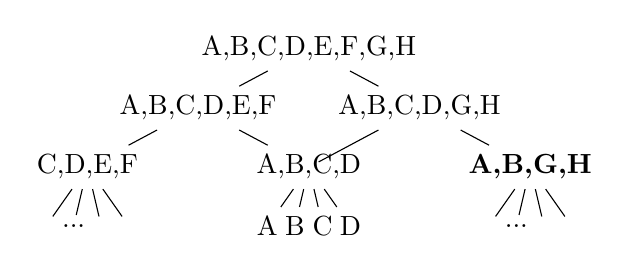
\begin{tikzpicture}
[level 1/.style={sibling distance=8em},
 level 3/.style={sibling distance=1em}, level distance=0.75cm]
    \tikzstyle{n}=[draw, fill, circle]

    \node (a) at (0,0) {A,B,C,D,E,F,G,H}
        child { node {A,B,C,D,E,F} 
            child { node {C,D,E,F}
                child {node { }}
                child {node {...}}
                child {node { }}
                child {node { }}
                } 
            child { node (shared) {A,B,C,D}
                child {node {A}}
                child {node {B}}
                child {node {C}}
                child {node {D}}
                } 
            }
        child { node {A,B,C,D,G,H} 
            child { node { } }
            child { node {{\bf A,B,G,H}} 
                child {node { }}
                child {node {...}}
                child {node { }}
                child {node { }}
            }
        };
\end{tikzpicture}
    \caption{}
\end{subfigure}
%
\begin{subfigure}{0.2\linewidth}\centering
    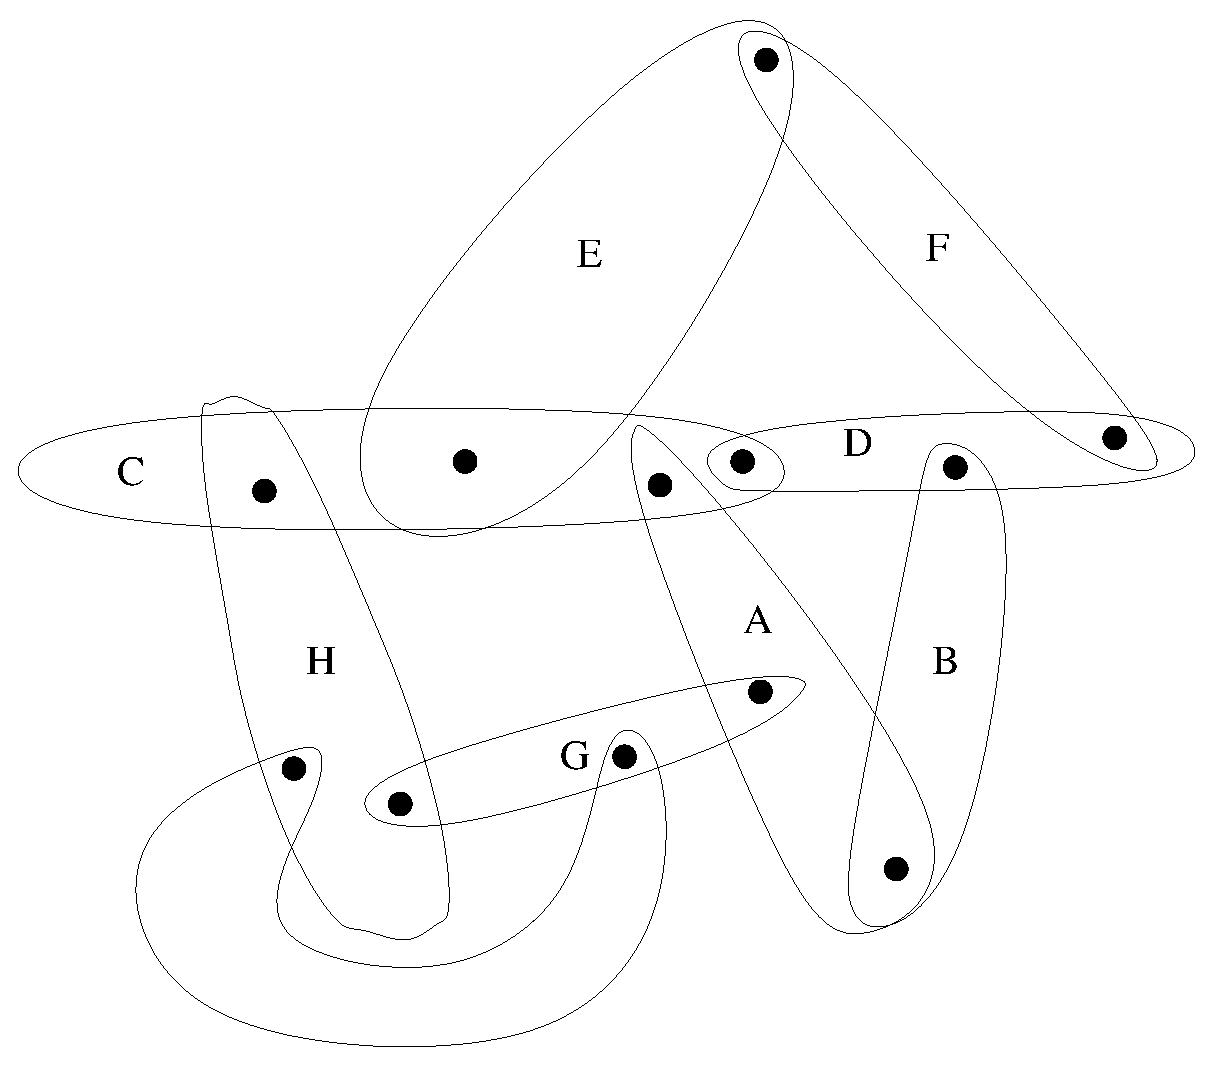
\includegraphics[width=\linewidth]{img/bodypin2}
    \caption{}
\end{subfigure}
%
\caption{(a) is a 1 dof body-pin qusec. (b) is the corresponding body-bar graph explained in Definition \ref{def:body-pin}. (c) is the 1 dof DR-plan for the graph. In this case, to obtain an isostatic system, we would need to add a body and 2 pins to one of the nodes in the second level. (d) is the result of adding one such body to the bold-faced node.}

\end{figure*}

\begin{theorem}
    There is a quadratic algorithm for the 1 dof optimal completion problem of Seciton \ref{sec:recomb} for body-pin and multi-triangle-pin qusecs.
\end{theorem}

\begin{proof}
    Suppose we are given a body-pin qusec and its corresponding body-bar graph $G$ and have obtained the DR-plan $T$. Each node of $T$ will then be a vertex maximal proper 1 dof subgraph of $G$. To make the entire graph wellconstrained, we can add a body (vertex) and pin it (add a 2-multiedge) to a node $b$ in $T$ such that the body is pinned to 2 separate children of $b$. From Remark \ref{rem:1dofcanon}, we know that the children can only be joined by a single pin or a subgraph, so we simply have to pin the new body to the 2 bodies joined by the pin or that are not in the intersecting graph. Doing so will ensure the following:

    \begin{itemize}
        \item All children of $b$ will remain 1 dof
        \item All ancestors of $b$ (including $b$) will now be wellconstrained
    \end{itemize}

    Then, we can form a valid isostatic DR-plan $T_b$ from $T$. In $T_b$, $b$'s children are now all of the leaf nodes of the subtree rooted at $b$ because no child of $b$ in $T$ is isostatic. Similarly, for any other node $w$ that is an ancestor of $b$, $w$'s children will be the node that leads to $b$, denoted $b'$, along with all of the other leaf nodes in the tree rooted at $w$ excluding $b'$. Then, for any node $b$ that we choose, $T_b$ is a valid DR-plan. Thus, if we want to minimize the size of our DR-plan, we simply need to take the $b$ that has the $T_b$ of smallest size. Running this algorithm in a brute force fashion is quadratic in the number of bodies of our given body-pin system.

    For the multi-triangle pin qusecs, we can do the same thing except we need to add a single triangle to one of the nodes to cause it to become isostatic.

    % For the 2 dof case, we can do something very similar, except instead of pinning a single body 2 times to a node, we can pin another body 2 times to a node. These can be the same node, and if it is the same node, we can find a wellconstrained DR-plan in quadratic time, we would just be doing the same thing as the 1 dof case.
\end{proof}

% THIS NEEDS SOME MORE THINKING. THERE ARE DIFFERENT TYPES OF CHILDREN NODES FOR THIS PART. NOT JUST THE TWO LISTED ABOVE

\begin{theorem}
    There is a \textcolor{red}{$O(?)$} algorithm for the 1 dof optimal completion problem of Seciton \ref{sec:recomb} for body-pin and multi-triangle-pin qusecs.
\end{theorem}

\begin{proof}
    We can do a similar algorithm to the 1 dof case, except we constrain a given node 2 times (by adding 2 triangles or 2 bodies and 4 pins). This causes the nodes along the path to the given node to become well-constrained while all others will be underconstrained. Thus, our DR-plan will have the same size as the 1 dof case. This is still a quadratic algorithm.


\end{proof}

An open question remains as to the complexity of the optimal completion problem when there are more than 2 dofs. For higher number of dofs, the $(l,k)$ characterization is no longer matroidal.
